
\begin{frame}{Following the time evolution of the interaction}
		
		{\scriptsize Normalized quantities: summing across the outflow boundary and divided by the jet values}
	\begin{columns}
	 \begin{column}{0.5\textwidth}
      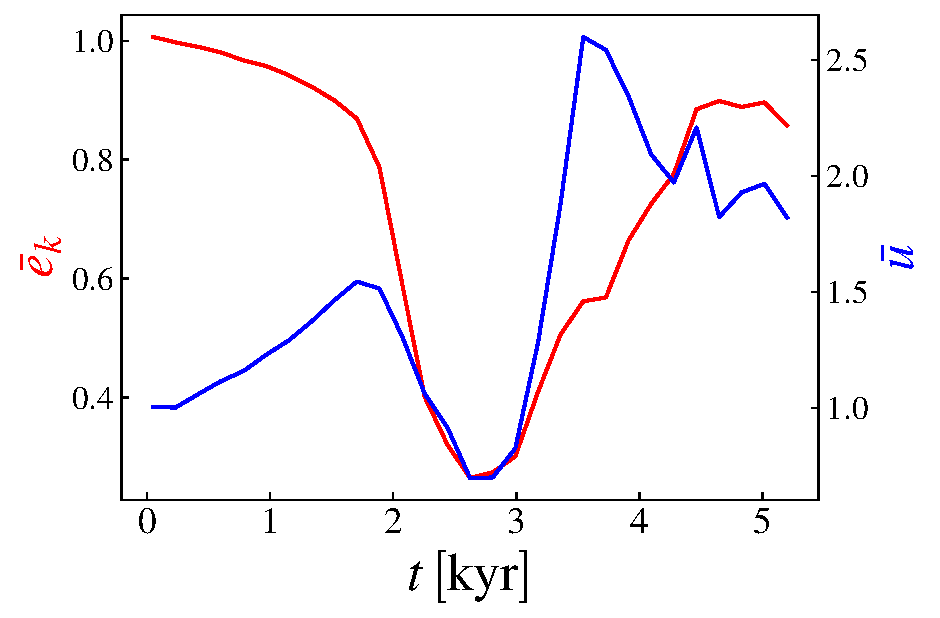
\includegraphics[width=\linewidth]{images/evolution_integrated_xz_u_uk_2_riot.pdf}
     \end{column}
	 \begin{column}{0.5\textwidth}
		{\footnotesize
		\begin{block}{Kinetic and internal energy densities}
			\begin{itemize}
				\item Global drop for both energies
				\item $u \nearrow$ whith the swept heated ejecta 
				\item $e_k \nearrow$ with the heavy matter incorporated
			\end{itemize}
		\end{block}}
	\end{column}
	\end{columns}
	\begin{columns}

	   \begin{column}{.5\textwidth}

      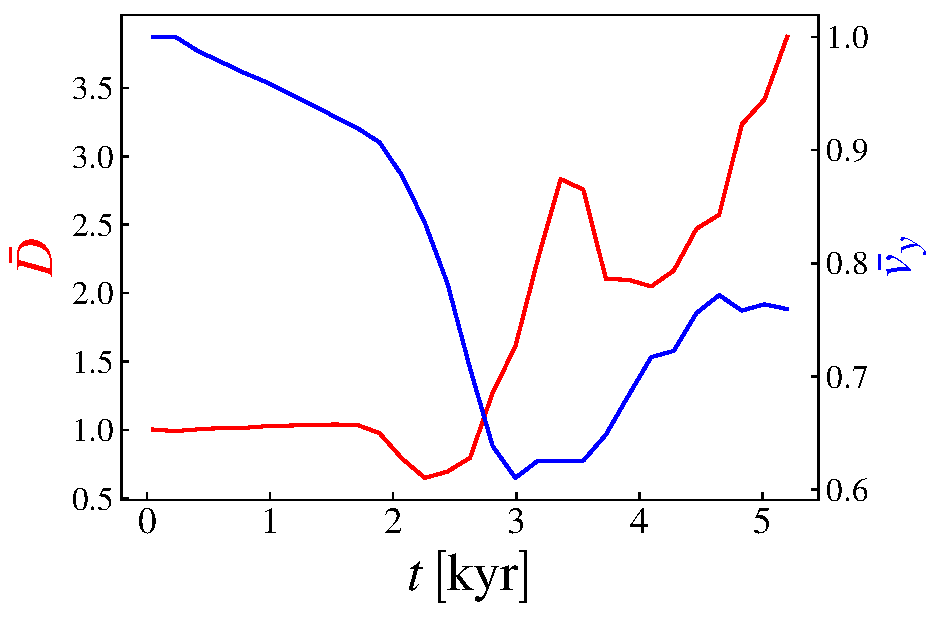
\includegraphics[width=\linewidth]{images/evolution_integrated_xz_d_vy_2_riot.pdf}
	   \end{column}
	   \begin{column}{.5\textwidth}
		{\footnotesize
		\begin{block}{Lab frame density and axial velocity}
			\begin{itemize}
				\item $D \nearrow$ with the entrainment of the ejecta
				\item $v_y \searrow$ with the disruption then $\nearrow$ with the reacceleration
			\end{itemize}
		\end{block}}
	   \end{column}
	\end{columns}
\end{frame}

\begin{frame}{RHD equations}
\begin{columns}
\begin{column}{0.5\textwidth}
Stress-energy tensor : $T^{\mu \nu} = \rho h u^{\mu} u^{\nu} + p g^{\mu\nu}$ \\
We use the Ratpenat code which solves the conservation equations with high-resolution shock-capturing method
{\small
\begin{align*}
 \frac{\partial \bf{U}}{\partial t} + \frac{\bf{F^{i}}}{\partial x^{i}} = 0
\end{align*}
}
Where $\bf{U}=(D,S^{j},\tau)^{T}$ and

\[
\bf{F} =
\begin{pmatrix}
  Dv^{i} \\
  S^{j}v^{i}+p\delta^{ij} \\
  S^{i}-Dv^{i} \\
\end{pmatrix}
\]

\end{column}
\begin{column}{0.5\textwidth}
The conservative variables are related to the primitive one \\
\begin{exampleblock}{}
The rest mass density $D = \rho \Gamma $ \\
The density momentum $S^{i} = \rho h \Gamma^{2} v^{i}$ \\
The energy density $\tau = \rho h\Gamma^{2} - p - D$ \\
\end{exampleblock}

Where we can define the 4-vector velocity $u^{\alpha} = \Gamma(1,v^{i})$ \\
The specific enthalpy $h=1+\epsilon/c^{2}+p/(\rho c^{2})$ \\
And the Lorentz factor $\Gamma = \frac{1}{\sqrt{1-v^{i}v_{i}/c^{2}}}$
\end{column}
\end{columns}
\end{frame}

\begin{frame}{RMHD equations}

\begin{columns}
\begin{column}{0.5\textwidth}
{\small
\begin{align*}
 \frac{\partial \bf{U}}{\partial t} + \frac{\bf{F^{i}}}{\partial x^{i}} = 0
\end{align*}
}
	Where $\bf{U}=(D,S^{j},\tau,B^{j})^{T}$ and

\[
\bf{F} =
\begin{pmatrix}
  Dv^{i} \\
	\rho h^{*}W^{2}*v^{j}v^{i}+p^{*}\delta^{ij} - b^{i}b^{j} \\
	\rho h^{*}W^{2}v^{i}-b^{0}b^{i} - \rho W v^{i}\\
	v^{i}B^{j}-B^{i}v^{j}\\
\end{pmatrix}
\]

\end{column}
\begin{column}{0.5\textwidth}
And we can define the other variables: \\
	4-vector velocity $u^{\alpha} = \Gamma(1,v^{i})$ \\
	4-vector magnetic field where $b^{0} = W(\mathbf{v}\cdot\mathbf{B})$ \\
	$b^{i} = \frac{B^{i}}{W} + v^{i}b^{0}$ \\
	And the magnetic pressure would be $|b|^{2} = \frac{B^{2}}{W^{2}} + (\mathbf{v}\cdot\mathbf{B})^{2}$ \\
	The specific enthalpy $h^{*}=1+\epsilon+p/(\rho)+|b|^{2}/\rho$ \\
	The total pressure $p^{*} = p_g + p_{mag} = p + |b|^{2}/2$ \\
	
\end{column}
\end{columns}


\end{frame}
